\section{Benchmarks and GRMHD codes}
In the following sections, the solution of various academic benchmark
scenarios is demonstrated. These solutions have been obtained with the
path-conservative ADER-DG scheme presented in section \ref{sec:dg}.

%\subsection{The GRMHD PDE and its implementation}
In the \code{ExaHyPE} code, the full set of GRMHD equations
on dynamical spacetime with divergence
cleaning is implemented. The evolution quantities are given by
$Q_\grmhd=(D,S_j,\tau,B^i,\phi)$ and the PDE \eqref{intro:ncp} terms
are given by \footnote{
  The PDE presented in \cite{Fambri2018} completely avoids the
  algebraic source $S=0$, since all tests presented in the paper
  are carried out with stationary spacetime. Thus the hydrodynamic
  source term from Section~\ref{sec:Cowling-approx} is shown in
  \cite{Fambri2018}.
}
\begin{align}\label{eq.grmhd.summary}
	F^i(Q) &=
	\begin{pvector}
		\text{fluxes for } D \\
		\text{fluxes for } S_j \\
		\text{fluxes for } \tau \\
		\text{fluxes for }  B^j \\
		\text{fluxes for } \phi
	\end{pvector}
	=
	\begin{pvector}
		w^i D \\
		\alpha W^i_j - \beta^i S_j \\
		\alpha (S^i - v^i D) - \beta^i \tau \\
		w^i B^j - v^j B^i - B^i \beta^j \\
		\alpha B^i - \phi \beta^i
	\end{pvector}
	,
	\\
    B^{ij} \partial_i Q_j &=
	\begin{pvector}
	0
	\\
	- \frac \alpha2 S^{lm} \partial_j \gamma_{lm} - S_k \partial_j \beta^k + E \partial_j \alpha
	\\
	S^i \partial_i \alpha
	\\
	B^i \partial_i \beta^j + \alpha \gamma^{ij} \partial_i \phi \\
	\phi \partial_i \beta^i
	+ \frac 12 \phi \gamma^{ij} \beta^k \partial_k \gamma_{ij}
	- B^i \partial_i \alpha
	\end{pvector}
	,\,
	S =
	\begin{pvector}
	0
	\\
	0
	\\
	\alpha S^{ij} K_{ij}
	\\
	0
	\\
	- \alpha \kappa \phi
	\end{pvector}
	.
	\nonumber
\end{align}

The numerical code consists of three parts: The fundamental AMR code,
the numerical scheme which can solve a generic prototypic PDE
(see in general Chapter \ref{chapter:numerics}), and the particular PDE
parts, provided in \ref{eq.grmhd.summary}. Such an implementation requires
to perform a primitive recovery (Section \ref{sec:c2p}) at every evaluation
of $F^i$, $B^{ij}$ and $S$. 

\subsection{Benchmark description}
%\newcommand{\yes}{\Checkmark}
\newcommand{\yes}{\cmark}
\newcommand{\no}{\xmark}
\begin{table*}[t]
	\begin{tabularx}{\textwidth}{lXcccc}
		\toprule
		%        &      &                 &        & \multicolumn{2}{c}{Spacetime} \\
		%\cmidrule{5-6}
		Section & Name of Test (Initial Data)
		& BC
		& $\vec B \neq 0$ & Smooth & 
		Spacetime \\
		\midrule
		\ref{sec:conv} & \nameref{sec:conv} & exact & \no & \yes & curved \\
		\ref{sec:2D_torus_interior} & \nameref{sec:2D_torus_interior} & exact & 
		\no & \yes & curved \\
		\ref{sec:3D_Michel} & \nameref{sec:3D_Michel} & exact & \yes & \yes & 
		curved \\
		\ref{sec:grmhd-riemann-problems} & \nameref{sec:grmhd-riemann-problems} 
		& exact & \yes & \no & flat \\
		\ref{sec:2d-magnetic-loop} & \nameref{sec:2d-magnetic-loop} & periodic 
		& \no & \no & flat \\
		\ref{sec:2d-blast-wave} & \nameref{sec:2d-blast-wave} & outflow & \no & 
		\no & flat  \\
		\ref{sec:orszag-tang} & \nameref{sec:orszag-tang} & periodic & \no & 
		\no & flat \\
		\ref{sec:full_torus} & \nameref{sec:full_torus} & exact & \yes & \no & 
		curved \\
		\ref{sec:3d-torus-gr} & \nameref{sec:3d-torus-gr} & exact & \yes & \no 
		& curved \\
		\ref{sec:tov} & \nameref{sec:tov} & outflow & \yes & \no & curved \\
		\bottomrule
	\end{tabularx}
	\caption[
	  Overview of hydrodynamic benchmarks presented in chapter 
	  \ref{chapter:hydro}
	]{Overview of hydrodynamic benchmarks presented in the following
		sections. The columns are explained in the main text.
     }%
	\label{table:benchmark-overview}
\end{table*}

Table \ref{table:benchmark-overview} provides an overview about the
benchmarks which are presented on the next pages. The tests require either
one, two or three spatial dimensions \footnote{
  Since \code{ExaHyPE} supports only two and three dimensional setups,
  one dimensional tests are performed in two dimensions straightforward
  as setting the initial data $Q_0(x,y) = Q_0(x)$.
}. Some tests only cover the hydrodynamic part of the equations and set 
the magnetic field $\vec B=0$. Furthermore, ``smooth flows'' are
distinguished from ``non-smooth flows''. \emph{Smoothness} is defined
as having continous initial data which can be well-represented by DG
polynomials and do not require limiting. For smooth flows, the actual
convergence order of the scheme can be measured (and is provided). For
non-smooth flows, the ability of the code to handle accurately shocks
and large gradients will be illustrated.
%
Unless stated otherwise, all tests share the following properties:
\begin{enumerate}[(i)]
	\item An ideal EOS is adopted with the adiabatic index has been chosen
	   equal to $\Gamma=4/3$.
	\item The refinement factor is always $\mathcal{R}=3$.
	\item Any method requiring ADER-DG limiting employs the second-order
	  MUSCL-Hancock TVD finite-volume method (described in section~\ref{sec:MUSCL}).
	\item As a Riemann solver, the
      the Rusanov (or local Lax-Friedrichs) approximate Riemann solver has been used.
    \item problems in curved spacetimes have been solved employing
      Kerr-Schild coordinates, either spherical or Cartesian.
\end{enumerate}
\todo[color=green]{HD Benchmarks: Could provide a schema figure of how to read a convergence table}%
At the spatial boundary interface $\partial \Omega$
(column ``BC'' in Table \ref{table:benchmark-overview}), either exact boundary
conditions are applied (\ie the initial conditions are used as external
domain boundary values) or ``copy boundary conditions'' with outflow
properties for hydrodynamical flows are applied (\ie the last internal
state vector is used as an external value).


%=============================================================
\section{Smooth special-relativistic benchmarks}
\label{sec:smooth}
%=============================================================

%We first test the high order of convergence of our ADER-DG schemes
%against three different scenarios in curved spacetimes given respectively
%by: i) the Michel accretion of gas onto a black hole in KS {spherical}
%(KSS) coordinates and in 2D); ii) a stationary non-selfgravitating fluid
%torus in equilibrium around a black hole, again in 2D; iii) the Michel
%accretion with a radial magnetic field in KS {Cartesian} (KSC)
%coordinates and in 3D.

To ensure that the flow is actually smooth, in the following tests we will
restrict our computational domain to regions that are fully filled with
fluid. In this way, after successively refining the mesh, we evaluate the
$L_2$ and $L_\infty$ error norms at different DG polynomial
degrees and mesh resolutions so as to to measure the convergence order of
our numerical implementation and compare it with the expected mathematical
one. Anticipating what will be shown in more detail in the following
sections, the numerical results {confirm} the high order of accuracy of
the presented numerical scheme. Indeed, using the results shown in Tables
\ref{tab:CTBondi3D} and \ref{tab:CTMichel2D} 
we can conclude that the ADER-DG
$\mathbb{P}_N$ method reaches its design accuracy $N+1$ in most cases.

%-------------------------------------------------------------
\subsection{Michel accretion onto a Schwarzschild black hole in 2D}
\label{sec:conv}
%-------------------------------------------------------------
%
\begin{marginfigure}
	\hspace*{-.5cm}
    \includegraphics[width=1.2\textwidth]{grmhd-paper-official/Michel_rho_vr.pdf}
    \caption[
      Michel accretion, \ownPub{Fambri2018}
    ]{ Numerical solution for the
      two-dimensional Michel accretion test in KSS coordinates obtained
      with our ADER-DG $\mathbb{P}_5$ at $t=100$. The numerical solution of
      density (black) and radial velocity (red) interpolated along $200$ points at
      $\theta=1.5$ are shown.}  \label{fig:Michel}
\end{marginfigure}
\begin{margintable}
		\resizebox{\linewidth}{!}{
			\begin{tabular}{ c r  cccc  }
				%% \hline
	    		%% \multicolumn{7}{c}{\textbf{2D Michel accretion in KSS 
     			%%coordinates --- ADER-DG-$\mathbb{P}_N$}} \\
				%%  \hline 
				%%       & & \multicolumn{4}{c}{$\rho$}&   \\
				%%      \cmidrule(lr){3-6} 
				\hline
				& $N_x$ &  $\mathcal{E}_{L_2}$ & $\mathcal{E}_{L_\infty}$ & $L_2$ & $L_\infty$  \\ % &Exp. \\ 
				\hline
				\multirow{4}{*}{\rotatebox{90}{{DG-$\mathbb{P}_1$}}}
				& 10	& 5E-05	& 9E-05	& --	&  --				 
				%\multirow{4}{*}{2}	 
				\\
				& 20	& 1E-05	& 2E-05	&  2.13	& 2.08	\\
				& 40	& 3E-06	& 5E-06	&  2.06	& 2.05	\\
				& 80	& 7E-07	& 1E-06	&  2.03	& 2.02		\\
				\cline{2-6}
				\hline
				\multirow{4}{*}{\rotatebox{90}{{DG-$\mathbb{P}_2$}}}
				&6	&  2E-05	& 3E-05		&   ---	&  ---	
				%&\multirow{4}{*}{3}
				\\
				&12	&  3E-06	& 4E-06		&  2.93	& 2.87	\\
				&18	&  1E-06	& 1E-06		&  2.93	& 2.91	\\
				&30	&  2E-07	& 3E-07		&  2.94	& 2.93	 \\
				\cline{2-6}
				\hline
				\multirow{4}{*}{\rotatebox{90}{{DG-$\mathbb{P}_3$}}}
				&4	&  3E-07	& 1E-06		&   ---	&  ---	
%				&\multirow{4}{*}{4}
				\\
				&6	&  5E-08	& 1E-07		&  4.65	& 4.59	 \\
				&8	&  1E-08	& 4E-08		&  4.21	& 4.51	\\
				&12	&  3E-09	& 8E-09		&  3.96	& 4.35	\\
				\cline{2-6}
				\hline
				\multirow{4}{*}{\rotatebox{90}{{DG-$\mathbb{P}_4$}}}
				&2	& 3E-06	& 5E-06	&  ---	&  ---	\\%&\multirow{4}{*}{5}\\
				&3	& 4E-07	& 5E-07	& 5.51	& 5.77	 \\
				&4	& 9E-08	& 1E-07	& 5.22	& 4.97	\\
				&5	& 2E-08	& 4E-08	& 5.18	& 4.93	\\
				\cline{2-6}
				\hline
				\multirow{4}{*}{\rotatebox{90}{{DG-$\mathbb{P}_5$}}}
				&2	&  6E-08	& 3E-08		&   ---	&  ---	
				%&\multirow{4}{*}{6}
				\\
				&3	&  4E-09	& 2E-09		&  6.68	& 6.50	 \\
				&4	&  6E-10	& 3E-10		&  6.31	& 6.30	\\
				&5	&  1E-10	& 1E-10		&  6.27	& 5.83	 \\ 
				\cline{2-6}
				\hline
				\multirow{4}{*}{\rotatebox{90}{{DG-$\mathbb{P}_6$}}}
				&2	& 1E-08	& 4E-09	&   ---	&  ---	\\%&\multirow{4}{*}{7}\\
				&3	& 4E-10	& 2E-10	&  7.81	& 7.21	 \\
				&4	& 5E-11	& 3E-11	&  7.43	& 6.72	\\
				&5	& 1E-11	& 8E-12	&  7.37	& 6.71	\\
				\cline{2-6}
				\hline	
			\end{tabular}
	}%resizebox
	\caption[
	Convergence table for 2D Michel accretion
	]{ $L_2$ and $L_\infty$ errors and
		convergence rates for the 2D Michel accretion in spherical
		Kerr-Schild coordinates for the ADER-DG-$\mathbb{P}_N$ scheme. We
		report the convergence results for the rest-mass density $\rho$ at
		$t=10$ up to $N=6$, and contrast the results with the expected
		rate. The domain has been chosen different (enlarged) for the cases
		$N=5$ and $N=6$ in order to keep away the numerical error from the
		machine limit. Similar results have also been obtained for all other
		flow variables.}\label{tab:CTMichel2D} 
\end{margintable}
%
As a first test of a smooth flow with an analytical solution we consider
the spherical transonic accretion of an isentropic fluid onto a
nonrotating black hole is known as {Michel solution}
\citep{Michel72}. For the sake of
completeness we give the explicit expressions of the lapse, the shift and
the spatial metric of a Kerr black hole with mass $M$ and spin $a$ in
{Cartesian} Kerr-Schild coordinates $\vec r = (x,y,z)$:
%
\begin{equation}
  \alpha = S^{-\halb}\,, \quad \beta^i = \frac{2 H}{S} l_i\,, \quad H = M
  \frac{r^3}{r^4 + a^2 z^2}\,, \quad S = 1 + 2 H\,,
\end{equation}
\begin{equation} 	
	\gamma_{ij} = \left( \begin{array}{ccc} 1 + 2 H l_x^2 & 2 H l_x
          l_y & 2 H l_x l_z \\ 2 H l_x l_y & 1 + 2 H l_y^2 & 2 H l_y l_z
          \\ 2 H l_x l_z & 2 H l_y l_z & 1 + 2 H l_z^2
	\end{array} \right)\,,
	\label{eq.kerr.metric}
\end{equation}
\begin{equation}
\text{with}\quad
  l_x := \frac{r x + a y}{r^2 + a^2}\,, \qquad l_y := \frac{r y - a
    x}{r^2 + a^2}\,, \qquad l_z := \frac{z}{r}
\end{equation}
\begin{equation}
\text{and}\quad
  r =
  \sqrt{ \frac{|\vec r|^2 - a^2}{2} + \sqrt{\left(\frac{|\vec r|^2 -
      a^2}{2}\right)^2 + z^2 a^2} }\,.
\end{equation}
%
Conversely, the Kerr metric in {spherical} Kerr-Schild coordinates
$(r,\theta,\phi)$ is given by \citep{Komissarov04}
%
\begin{equation}
  \alpha = (1+z)^{-\frac{1}{2}}, \quad \beta^i = \left( \frac{z}{1+z},0,0
  \right) , \quad
\end{equation}
\begin{equation}
	\gamma_{ij} = \left( \begin{array}{ccc} 1 + z & 0 & - a \sin^2
          \theta (1 + z) \\ 0 & \rho^2 & 0 \\ - a \sin^2 \theta (1 + z) &
          0 & {\Sigma} \sin^2 \theta/{\rho^2}
	\end{array} \right)\,,
	\label{eq.kerr.metric.spherical}
\end{equation}
\begin{equation}
  \text{with}\quad
	 \rho^2 := r^2 + a^2 \cos^2 \theta\,, \qquad z := \frac{2 r}{\rho^2}\,,
\end{equation}
\begin{equation} 
	\Delta := r^2 + a^2 - 2 M r\,, \qquad \Sigma = (r^2 + a^2)^2 - a^2
        \Delta \sin^2 \theta\,.
\end{equation}

The metric \eqref{eq.kerr.metric.spherical} without spin ($a=0$), with
black hole mass $M=1$ and (arbitrarily chosen) critical radius $r_c=8\,M$
and critical density $\rho_c M^2=1/16$ allows to determine the Michel solution
analytically \cite{Rezzolla_book:2013}.

This test was performed in spherical Kerr-Schild coordinates with a spatial
domain $(r,\theta)\in\Omega=[1.5,100]\times[0.15, 3.0]$, \ie the simulation
domain penetrates the event horizon but does not include the singularity.
The spatial domain is discretized with a uniform mesh of $200\times 32$ elements
and solved with the ADER-DG $\mathbb{P}_5$ scheme. A graphical representation
of the numerical results and their comparison with the analytic solution is
shown in Fig.~\ref{fig:Michel}, while the results of the convergence study are
provided in Table~\ref{tab:CTMichel2D}. Clearly, we can note an
excellent agreement between analytical and numerical solution and that
the latter converges at the expected and high order.

%-------------------------------------------------------------
\subsection{Torus interior around a Schwarzschild black hole in 2D}
\label{sec:2D_torus_interior}
%-------------------------------------------------------------
\begin{marginfigure}[-1cm]
 \includegraphics[width=\textwidth]{sven-torus/logrho.png}
 \caption[
   Rest mass density in thick torus spacetime, Matplotlib, \exclusive
 ]{
   Example of a thick torus configuration, two dimensional cut in the
   azimuth plane ($\theta=0$).
   Colour encodes the rest mass density $\rho$ (Logarithm of solar
   mass units) within the Roche lobe. Solid lines indicate equipotentials.
 }
\end{marginfigure}
In this test, a numerical convergence study of a stationary solution of
a thick disk (also refered to as Polish donut or axisymmetric test-fluid
torus) orbiting around a Schwarzschild black hole ($a=0$) of mass $M=1$
in 2D spherical Kerr-Schild coordinates. The theory of the equilibrium of these
non-selfgravitating fluids in GRHD has been first proposed by
\cite{Abramowicz78, Kozlowski1978} and has been the subject of a vast
literature. 
{ For completeness, we give in the following a brief
description of the setup of the primitive
variables of this test problem, referring to
\cite{Font02a,Rezzolla_book:2013,Anton06,DelZanna2007} for details 
about a more
general configuration of the fluid, depending on the selected values of
physical parameters.
 
%For the chosen test configuration the initialisation of the primitive
%variables is also summarised in appendix \ref{sec:TorusIC}. The reader is referred to
%\cite{Rezzolla_book:2013,Anton06,DelZanna2007} for details about a more
%general configuration of the fluid, depending on the selected values of
%physical parameters.
}

\subsection*{Torus description}
\label{sec:TorusIC}
\begin{marginfigure}
	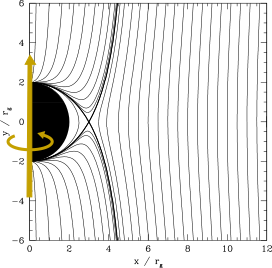
\includegraphics[width=\linewidth]{sven-torus/Zeipel-Zylinders.pdf}
	\caption[
	   Zeipel's cylinders, \modifiedAfter{Font02a}
	]{Surfaces with constant $\Omega=\Omega(\ell)$ are also refered to
	  as \emph{von Zeipel's cylinders}. Figure modified from \cite{Font02a}.
}
\end{marginfigure}
The acceleration experienced by a test fluid rotating around around a
Schwarz\-schild black hole (cylindrical symmetry) can be cast into the
following differential equation
%
\begin{align}
\label{eq:diff}
d \log |u_t| - \left(\frac{\Omega}{1-\Omega \ell} \right) d \ell +
\frac{d p}{\rho h} = 0\,, 
\end{align}
\begin{align}
\label{eq:Omega}
\text{with specific angular momentum }\quad
\ell(r,\theta)&:=-\frac{u_\phi}{u_t} \,, \\
\text{and (coordinate) angular velocity} \quad \Omega(r,\theta)&:=
\frac{u^\phi}{u^t} \,,
%% =
%% - \frac{ g_{t\phi} + g_{\phi\phi}
%%   \Omega}{g_{tt} + g_{t\phi} \Omega} \label{eq:ell}
%% \\% \quad \text{and}
%% \quad \Omega(r,\theta)&:= \frac{u^\phi}{u^t} = - \frac{ g_{t\phi} + g_{tt}
%%   \ell}{g_{\phi\phi} + g_{t\phi} \ell}\,, \label{eq:Omega}
\end{align}
%
For {barotropic} fluids the last differential
on the right in Eq. (\ref{eq:diff}) is exact, \ie one can define the
{effective potential} $\mathcal{W}$ via
%
\begin{align}
\mathcal{W}-\mathcal{W}_{\text{in}} := - \int_0^p \frac{d \tilde{p}}{\rho
	h}=
%% \mathcal{W} - \mathcal{W}_{\text{in}} =
\log |u_t| -
\log|(u_t)|_{\text{in}} - \int \limits_{\ell_{\text{in}}}^{\ell}
\frac{\Omega d\tilde{\ell}}{1-\Omega \tilde{\ell}}\,.
\end{align}
%
%% After integration of Eq. (\ref{eq:diff}), one obtains
%% \begin{align}
%%   \mathcal{W} - \mathcal{W}_{\text{in}} = \log |u_t| -
%%   \log|(u_t)|_{\text{in}} - \int \limits_{\ell_{\text{in}}}^{\ell}
%%   \frac{\Omega d\tilde{\ell}}{1-\Omega \tilde{\ell}}\,.
%% \end{align}
%
In the case considered here, the specific angular momentum is assumed
to be constant $\ell=\ell_0=\text{const.}$, so that it is possible to obtain
an explicit and simplified expression for the potential
%
\begin{align}
\mathcal{W}(r,\theta) = \log |u_t|\,,
\label{eq:effPot}
\end{align}
%
where, for a Schwarzschild black hole, one has
%
\begin{align}
u_t = -r \sin \theta \left( \frac{r-2}{r^3 \sin^2 \theta - \ell^2
	(r-2)}\right)^{\frac{1}{2}}\,.
\end{align}

In the axisymmetric equilibrium torus, there are some special radial
positions in the equatorial plane ($\theta = \pi/2$) that are worthwhile
recalling: the {inner} and {outer} edge of the torus $r_{\text{in}}$ and
$r_{\text{out}}$; the radial position of the {cusp}, $r_{\text{cusp}}$;
the radial position of the maximum pressure peak, $r_{\text{c}}$, which
is the {center of the torus}; the radial position of the 
``{marginally stable}'' and ``{marginally bound}'' orbit, $r_{\text{ms}}$
and $r_{\text{mb}}$. The cusp position $r_{\text{cusp}}$ and the centre
$r_{\text{c}}$ can be identified as the local extrema of the effective
potential, but also by the condition $\ell_K=\ell_0$, where $\ell_K$ is
the {Keplerian specific angular momentum} which is given by $\ell^2_K(r)
:= M r^3 / (r - 2M)^2$. Similarly, also $r_{\text{ms}}$ and
$r_{\text{mb}}$ are identified by the condition $\ell_K =
\ell_{\text{ms}}$ and $\ell_K=\ell_{\text{mb}}$. For a Schwarzschild
(nonrotating) black-hole: $\ell_{\text{ms}} = (3\sqrt{6}/2) M$ and
$\ell_{\text{mb}} = 4 M$, so that the corresponding to the radial
positions are $r_{\text{ms}} = 6 M$ and $r_{\text{mb}} = 4 M$.

\begin{marginfigure}
	\includegraphics[width=\textwidth]{sven-torus/Geometrically-thick-torus.pdf}
	\caption[
	Torus potentials, \modifiedAfter{Font02a}
	]{Torus potentials, Figure modified after \cite{Font02a}}
\end{marginfigure}

Finally,
the inner and outer radial position, $r_{\text{in}}$ and
$r_{\text{out}}$, can be estimated by the condition $\Delta \mathcal{W}
:= \mathcal{W}_{\text{in}} - \mathcal{W}_{\text{cusp}} = 0$. Indeed,
whenever $\Delta \mathcal{W}>0$ the orbit of the corresponding fluid
particle is open, whenever $(\mathcal{W}_{\text{c}} -
\mathcal{W}_{\text{in}}) < \Delta \mathcal{W}<0$ the orbits are
closed. The spatial volume delimited by the widest closed equipotential
surface of the torus, \ie $\mathcal{W}=\mathcal{W}_{\text{cusp}}$ is
named as the ``{Roche lobe}'' of the torus. Using these definitions,
several constraints need to be satisfied: first, the cusp
$r_{\text{cusp}}$ must necessarily be located within $r_{\text{mb}}$ and
$r_{\text{ms}}$, and the inner edge $r_{\text{in}}$ can be located
anywhere within $r_{\text{cusp}}$ and $r_{\text{c}}$. For isentropic
fluids obeying the {polytropic} EOS ($p = K \rho^{\Gamma}$),
an analytical expression for the rest-mass density exists and takes the
form
%
\begin{align}
\rho(r,\theta) = \left[\frac{\Gamma - 1}{K \Gamma} \left( \exp(
\mathcal{W}_{\text{in}} - \mathcal{W}(r,\theta) ) -
1\right)\right]^{1/\left(\Gamma - 1\right)} \label{eq:rhotorus}
\end{align}

%For the chosen test configuration the initialisation of the primitive
%variables is briefly summarised below. The reader is referred to
%\cite{Rezzolla_book:2013,Anton06,DelZanna2007} for details about a more
%general configuration of the fluid, depending on the selected values of
%physical parameters.

After choosing the value of the polytropic constant $K$, polytropic
exponent $\Gamma$, the specific angular momentum $\ell_0$, and the
potential gap $\Delta \mathcal{W}$, then the Keplerian points are
estimated after ensuring the following scalar equalities: for the radial
cusp position $r_{\text{cusp}}$, 
\begin{marginfigure}
	\includegraphics[width=\textwidth]{sven-torus/3d-torus.png}
	\caption[
	  3D plot of a NS-Torus spacetime, rendered with Visit, \exclusive
	]{
	  The theory of thick tori can also be applied to other spacetimes
	  with cylindrical symmetry, for instance to the sapcetime of a
	  neutron star (shown here in a surface countour plot of the rest
	  mass density $\rho$). This artificially created object
	  (linear superposition of two spacetimes) remains surprisingly
	  stable during evolution.
	}
\end{marginfigure}
%
\begin{align}
\ell_K(r) = \ell_0\,, \quad \text{with} \quad r_{\text{hor}}< r <
r_{\text{ms}}\,,
\end{align}
%
for the center $r_{\text{c}}$,  $r_{\text{hor}}$ being the radial position of the horizon,
%
\begin{align}
\ell_K(r) = \ell_0\,, \quad \text{with} \quad r_{\text{ms}} < r\,.
\end{align}
%
Then, the corresponding potentials $\mathcal{W}_{\text{cusp}}$. and
$\mathcal{W}_{\text{c}}$ are evaluated according to Eq.
(\ref{eq:effPot}). On the other hand, the effective potential at the
inner edge $\mathcal{W}_{\text{in}}$ is computed according to the
prescribed potential gap $\Delta \mathcal{W}$ after estimating
%
\begin{align}
(u_{t})_{\text{ in}} = (u_{t})_{\text{ cusp}} \;e^{\Delta \mathcal{W}}\,.
\end{align}
%
Then, since the fluid distribution is inside the Roche lobe, the inner
and outer edge positions $r_{\text{in}}$ and $r_{\text{out}}$ are
computed through the conditions
%
\begin{align}
u_t(r) &= (u_{t})_{\text{ in}} \quad \text{with} \quad r_{\text{cusp}} <
r < r_{\text{c}}\,,
\\
\text{and}\quad
u_t(r) &= (u_{t})_{\text{ in}} \quad \text{with} \quad r_{\text{c}} <
r\,,
\end{align}
respectively. The rest-mass density at the center $\rho_{\text{c}}$ is
provided directly by the analytical solution (\ref{eq:rhotorus}), the
corresponding pressure $p_{\text{c}}$ through the EOS.
Finally, for every spatial position
$(r,\theta)$ within the torus, \ie which fulfils the condition
%
\begin{align}
r>r_{\text{in}} \quad \text{and} \quad
\mathcal{W}<\mathcal{W}_{\text{in}}\,,
\end{align}
%
the angular velocity $\Omega(r,\theta)$ is computed through the
definition (\ref{eq:Omega}), the rest-mass density $\rho$ directly from
(\ref{eq:rhotorus}), and the velocity is given by
%Notice the Keplerian angular velocity is given by
%\begin{align}
%\Omega_K(r) = M^{1/2}r^{-3/2}
%\end{align}
%% the main hydrodynamic quantities inside the torus can be expressed as
\begin{align}
%&\rho 	  = \rho_d\\
%&p 		 = p_d \\
&(v^r ,v^\theta ,v^{\phi} ) = \left( \frac{\beta^r}{\alpha} , 0 ,
\frac{1}{\alpha}(\Omega + \beta^\phi) \right)\,.
\end{align}




\subsection*{Torus evolution}
\begin{margintable}
	\resizebox{\linewidth}{!}{
		\begin{tabular}{ c r  cccc  }
			%% \hline
			%% \multicolumn{7}{ c }{\textbf{2D torus-interior problem in KSS coordinates --- ADER-DG-$\mathbb{P}_N$}} \\
			%%  \hline 
			%%       & & \multicolumn{4}{c}{$\rho$}&   \\
			%%      \cmidrule(lr){3-6} 
			\hline
			& $N_x$ &  $\mathcal{E}_{L_2}$ & $\mathcal{E}_{L_\infty}$ & $L_2$ & $L_\infty$  \\ % &Exp. \\ 
			\hline
			\multirow{4}{*}{\rotatebox{90}{{DG-$\mathbb{P}_1$}}}
			& 10	& 5E-07	& 2E-06	 &  ---	&  ---	 \\ %&\multirow{4}{*}{2}	 
			& 20	& 1E-07	& 9E-07	 	& 1.68	& 1.55	\\ % &\\
			& 30	& 7E-08	& 4E-07	 	& 1.83	& 1.84	\\ %&\\
			& 40	& 4E-08	& 2E-07	 	& 1.86	& 1.92	\\ %&\\
			\cline{2-6}
			\hline
			\multirow{4}{*}{\rotatebox{90}{{DG-$\mathbb{P}_2$}}}
			&10	&   5E-08	& 1E-07	 &  ---	&  ---	  \\ %&\multirow{4}{*}{3}\\
			&15	&   1E-08	& 5E-08	 & 2.65	& 2.47	 \\  %&\\
			&20	&   8E-09	& 2E-08	 & 2.64	& 2.78	  \\ %&\\
			&30	&   2E-09	& 7E-09	 	& 2.70	  & 2.70 \\  %&\\
			\cline{2-6}
			\hline
			\multirow{4}{*}{\rotatebox{90}{{DG-$\mathbb{P}_3$}}}
			&8	&   3E-09	& 1E-08	 &  ---	&  ---	\\  %&\multirow{4}{*}{4}\\
			&10	&   1E-09	& 9E-09	 & 3.69	& 3.13	\\  %& \\
			&15	&   3E-10	& 2E-09	 & 4.04	& 3.79	 \\ %&\\
			&20	&   1E-10	& 7E-10	 	& 3.69	 & 3.64\\ %&\\
			\cline{2-6}
			\hline
			\multirow{4}{*}{\rotatebox{90}{{DG-$\mathbb{P}_4$}}}
			&2	&   1E-07	& 3E-07	 	&  ---	&  ---	\\  %&\multirow{4}{*}{5}\\
			&3	&   1E-08	& 3E-08	 	& 5.57	& 5.44 \\ 	% &\\
			&4	&   3E-09	& 1E-08	 	& 4.10	& 4.29	\\  %&\\
			&5	&   1E-09	& 5E-09	 	& 4.08	& 3.04	\\  %&\\
			\cline{2-6}
			\hline	
		\end{tabular}
	} % end of resizebox
	\caption[
	Convergence table for 2D spherical Kerr-Schild torus
	]{  $L_2$ and $L_\infty$ errors and
		convergence rates on the rest mass density $\rho$
		for the 2D torus-interior problem in spherical Kerr-Schild
		coordinates for the ADER-DG-$\mathbb{P}_N$ scheme. We report the
		convergence results for the rest-mass density $\rho$ at $t=10$ up to
		$N=4$. The expected convergence rate is always $N+1$. Similar
		results have also been obtained for all other hydrodynamic variables. } 
	\label{tab:CTTorus}
\end{margintable}

The free parameters of the problem have been chosen to be a specific
angular momentum of $\ell_0 = 3.8$, a potential gap $\Delta W = -
10^{-3}$ (inside and nearly filling its {Roche lobe}). The polytropic
constant and exponent have been chosen equal to $K=0.0496$ and
$\Gamma=4/3$, respectively.

Also in this case, for a rigorous testing of the convergence order we
have simulated only an inner portion of the torus which is fully filled
by fluid, namely, the one covered by the coordinate patch
$(r,\theta)\in\Omega=[7,10.5]\times[1.47,1.67]$. The corresponding
measured convergence order after evolving the set of the GRHD equations
in spherical Kerr-Schild coordinates are reported in Table \ref{tab:CTTorus}, once
again showing the expected high order of convergence of our ADER-DG
scheme. We conclude this test by remarking that torus simulations where
the torus is fully contained in the computational domain, which therefore
includes also a region set to {atmosphere}, will be presented in
Sec. \ref{sec:full_torus}.

\begin{figure*}
	\begin{center} 
		%\includegraphics[width=0.49\textwidth]{grmhd-paper-official/MichelWithB_3D_KSC.pdf}
		\includegraphics[width=0.49\textwidth]{grmhd-paper-official/MichelWithB_3D_KSC_b.pdf}
		\includegraphics[width=0.49\textwidth]{grmhd-paper-official/MichelWithB_3D_KSC_rhoBxVx.pdf}
		\caption[
		Michel accretion, 3D \ownPub{Fambri2018}
		]
		{  Numerical solution for the 3D Michel
			accretion test with radial magnetic field in KSC coordinates
			obtained with our ADER-DG $\mathbb{P}_3$ at $t=20$. \textit{Left
				panel:} 3D visualization of the numerical solution and mesh: the
			space elements at $y<0$ are artificially blanked (not-visible), at
			$y>0$ are coloured by the rest-mass density. Moreover, the computed
			density is shown also along the 2D cut-plane $y=x\leq0$ together
			with the stream-traces of the magnetic field. \textit{Right panel:} numerical
			solution interpolated along $200$ points at $z=0$ and $y=x$ for the
			rest-mass density (red), the $x$ component of the velocity (green) and
			magnetic field (blue) vectors are plotted next to the analytical
			solution. The numerical domain is $\bm{x} \in \Omega = [-5,
			5]^3$. 
     		Published in \cite{Fambri2018}.
	}\label{fig:Michel3D}
	\end{center}
\end{figure*}

%-------------------------------------------------------------
\subsection{3D Michel accretion with radial magnetic field}
\label{sec:3D_Michel}
%-------------------------------------------------------------
This is the 3D version of the similar test presented in
Sec. \ref{sec:2D_torus_interior}, with the addition of one spatial
dimension (corresponding to the azimuthal Killing vector) and of a
{radial magnetic field}. Although such a magnetic field is unphysical,
since it leads to a nonzero divergence and hence to the presence of a
{magnetic monopole}, it is nevertheless widely used for testing GRMHD
codes \cite{Etienne:2010ui}. Here, we use it to test the
convergence order of our high-order method by considering also the
magnetic component of the set of partial differential equations. In
addition, to stress-test our numerical infrastructure, we have employed
for this test 3D Cartesian KS coordinates, so that the magnetic field
lines are not aligned with any of the coordinate axis.
The chosen contravariant components of the radial magnetic field
take the form
%
\begin{align}
  B^i(\boldsymbol{x},t) = \gamma^{-\frac{1}{2}} M^2 B_0 \frac{x^i}{r^2}\,,
  ~\text{ with }~
  B_0 =
  \frac{2.688}{M}\left(\frac{b^2}{\rho}\right)_{\text{hor}}^{\frac{1}{2}}\,,
\end{align}
%
where the black-hole mass is again set to $M=1$ and $b^\mu$ is the
magnetic field measured by the Lagrangian observer comoving with the
fluid, \ie
\begin{align}
b^\mu := \frac{ \left(\delta^\mu_\nu + u^\mu u_\nu\right) B^\nu}{ -n_\nu
  u^\nu}\,.
\end{align}

\begin{margintable}[1cm]
	\resizebox{\linewidth}{!}{
		\begin{tabular}{ c r  cccc }
			%% \hline
			%% \multicolumn{7}{c}{\textbf{3D Michel accretion with radial magnetic 
			%%field }} \\
			%% \multicolumn{7}{c}{\textbf{in KSC coordinates --- 
			%%ADER-DG-$\mathbb{P}_N$}} \\
			%%  \hline 
			%%       & & \multicolumn{4}{c}{$B^x$}&   \\
			%% \cmidrule(lr){3-6} 
			\hline
			& $N_x$ &  $\mathcal{E}_{L_2}$ & $\mathcal{E}_{L_\infty}$ & $L_2$ & 
			$L_\infty$  \\% & $X$ \\ 
			\hline
			\multirow{4}{*}{\rotatebox{90}{{DG-$\mathbb{P}_1$}}}
			& 10	&	6E-04	&	2E-04	  &---  &--- 
			\\%&\multirow{4}{*}{2}\\
			& 20	&	1E-04	&	8E-05		&	1.9	&	1.3\\
			& 30	&	7E-05	&	4E-05		&	2.0	&	1.6\\
			& 40	&	4E-05	&	2E-05		&	2.0	&	1.8	\\
			%\cline{2-6}
			\hline
			\multirow{4}{*}{\rotatebox{90}{{DG-$\mathbb{P}_2$}}}
			&10&	3E-05	&	2E-05	&---	&--- 	
			\\%&\multirow{4}{*}{3}\\
			&15&	1E-05	&	7E-06		&	2.5	&	2.9\\
			&20&	6E-06	&	3E-06		&	2.4	&	2.4\\
			&30&	2E-06	&	1E-06		&	2.4	&	2.4\\
			%\cline{2-6}
			\hline
			\multirow{4}{*}{\rotatebox{90}{{DG-$\mathbb{P}_3$}}}
			&8	&	1E-06	&	1E-06	&---	&--- 	
			\\%&\multirow{4}{*}{4}\\
			&10	&	6E-07	&	3E-07		&	4.4	&	5.0 \\
			&15	&	1E-07	&	6E-08		&	4.3	&	4.2\\
			&20	&	3E-08	&	1E-08		&	4.2	&	4.5\\
			%\cline{2-6}
			\hline
			\multirow{4}{*}{\rotatebox{90}{{DG-$\mathbb{P}_4$}}}
			&6	&	4E-07	&	4E-07	&---	&--- 	
			\\%&\multirow{4}{*}{5}\\
			&8	&	1E-07	&	9E-08		&	5.0	&	5.0 \\
			&12	&	1E-08	&	1E-08		&	5.0	&	5.1\\
			&16	&	3E-09	&	2E-09		&	5.0	&	5.3\\
			%\cline{2-6}
			\hline
			\multirow{4}{*}{\rotatebox{90}{{DG-$\mathbb{P}_5$}}}
			&4	&	1E-07	&	3E-07	&---	&---  \\%&\multirow{4}{*}{6}\\
			&6	&	1E-08	&	3E-08		&	6.5	&	5.8 \\
			&8	&	2E-09	&	6E-09		&	5.9	&	6.1\\
			&10	&	6E-10	&	1E-09		&	5.8	&	6.1\\ 
			%\cline{2-6}
			\hline
			\multirow{4}{*}{\rotatebox{90}{{DG-$\mathbb{P}_6$}}}
			&6	&	1E-06	&	1E-06	&---	&--- 	
			\\%&\multirow{4}{*}{7}\\
			&8	&	1E-07	&	3E-07		&	6.9	&	5.2 \\
			&10	&	4E-08	&	1E-07		&	6.3	&	5.7\\
			&12	&	1E-08	&	3E-08		&	6.1	&	5.9\\
			%\cline{2-6}
			\hline	
		\end{tabular}
	} % end of resizebox
	\caption[
	Convergence table for 3D Michel accretion
	]{ $L_2$ and $L_\infty$ errors and
		convergence rates for the 3D Michel accretion with radial magnetic
		field in Cartesian Kerr-Schild coordinates for the
		ADER-DG-$\mathbb{P}_N$ scheme. We report the convergence results for
		the magnetic field component $B^x$ at $t=10$ up to $N=6$, and contrast
		the results with the expected rate. Similar results have also been
		obtained for all other flow variables. } \label{tab:CTBondi3D}
\end{margintable}

The spatial domain is in this case given by $(x,y,z)\in\Omega=[-5,+5]^3$
and is partitioned with a uniform mesh of $30^3$ elements, where we have
employed a very simple {cubic excision} to avoid the singularities at the
coordinates' origin location of the black hole as shown in the left panel
of Fig. \ref{fig:Michel3D}. At the excision boundary, we impose the exact 
solution of the problem as boundary condition in all variables. 

After adopting a ratio $(b^2/\rho)_{\text{hor}}=4$ at the horizon, the
results of the convergence study are presented in Table
\ref{tab:CTBondi3D}, while graphical representation of the numerical
results is offered in the right panel of Fig. \ref{fig:Michel3D}, which
reports the numerical solution interpolated along $200$ points at $z=0$
and $y=x$ for the rest-mass density and the $x$-component of the velocity
and of the magnetic field vectors as plotted against to the analytical
solutions. Clearly, also in this case the numerical solution is shown to
converge at the expected order of accuracy, confirming the validity of
our implementation in the presence of a magnetic field and of a
nontrivial coordinate mapping.


%=============================================================
\section{Non-smooth special-relativistic benchmarks}
\label{sec:discontinuous_sr}
%=============================================================

\begin{margintable}
\begin{center} 
\resizebox{\linewidth}{!}{
\begin{tabular}{lcclcc} %
	\toprule
	&\multicolumn{2}{c}{RP1} && \multicolumn{2}{c}{RP2} \\
	\cmidrule{2-3} \cmidrule{5-6}
	& $x>0$ & $x\leq 0$ && $x>0$ & $x\leq 0$ \\
	\midrule
    $\rho$ & 0.125 & 1.0 && 1.0   & 1.08 \\
    $v_x$  & 0     & 0   && -0.45 & 0.40 \\
    $v_y$  & 0     & 0   && -0.2  & 0.3  \\
    $v_z$  & 0     & 0   &&  0.2  & 0.2  \\
    $p$    & 0.1   & 1.0 &&  1.0  & 0.95  \\
    $B^x$  & 0.5   & 0.5 &&  2.0  & 2.0   \\
    $B^y$  & -1.0  & 1.0 &&  -0.7 &  0.3  \\
    $B^z$  & 0     & 0   &&  0.5  & 0.3 \\
	\hline
\end{tabular} 
}% resizebox
\caption[
  Initial condition parameters for the MHD Riemann problem
]{Initial conditions of the MHD variables for the Riemann 
problems.}\label{tab:RP1D}
\end{center}
\end{margintable}
\begin{margintable}
	\begin{center} 
			\begin{tabular}{ccc} %
				\toprule
				$\alpha$ & $\beta^x$ & $t_{\rm final}$ \\
				\midrule
                0.5 & 0   & 0.8 \\
                1 & 0 & 0.4 \\
                1 & 0.4 & 0.16 \\
                2 & 0 & 0.2 \\
				\hline
			\end{tabular} 
		\caption[
           Different Riemann problem curved background parameters
		]{Background spacetime and final time for different
		  Riemann problem runs.}\label{tab:RP1D-ADM}
	\end{center}
\end{margintable}

The tests considered in this section are considerably different from
those discussed so far in that they do not involve smooth flows and allow
therefore for the presence of nonlinear waves, either in the form of
shocks or of steep gradients as those present at the fluid interface with
an atmosphere.


\subsection{Riemann problems}\label{sec:grmhd-riemann-problems}
We start by considering two standard Riemann (or shock-tube) problems,
here referred to respectively as RP1 and RP2, and originally proposed in
the context of {special} relativistic MHD by \cite{Balsara2001}. Although
these tests are solved on flat spatial hypersurfaces, \ie
$\gamma_{ij}=\delta_{ij}$,
they employ different setups for the gauge variables, the
lapse function and the shift vector. In particular, Table \ref{tab:RP1D}
provides all the considered initial conditions for the MHD variables of
RP1 and RP2, while the lapse, the $x$-component of the shift and the
final time are chosen as in Table~\ref{tab:RP1D-ADM}.
The adiabatic index for RP1 and RP2 has been set to be $\Gamma=2$ and 
$\Gamma=5/3$, respectively.

For these tests, the HLL approximate Riemann solver has been used. Figure
\ref{fig:Balsara3D} offers a 3D view of the rest-mass density variable
for the proposed shock-tube problems and the corresponding AMR grid and
limiting status, for the case $\alpha=2$, obtained with our
ADER-DG-$\mathbb{P}_3$ scheme using a level-zero mesh of $40\times5$
space-elements onto with $\ell_{\text{max}}=2$ maximum refinement levels
are added, and an ADER-DG-$\mathbb{P}_5$ scheme on a level-zero grid of
$120\times5$ elements with one single refinement level
$\ell_{\max}=1$. The corresponding one-dimensional (1D) cuts relative to
the $\mathbb{P}_5$ solutions are presented instead in
Fig. \ref{fig:Balsara1P5} relatively to the test configurations
listed in Table \ref{tab:RP1D}; shown with solid
 lines are the corresponding
solutions from the exact Riemann solver of \cite{Giacomazzo:2005jy}.
{
In the presence of moving discontinuities, the expected order of convergence 
of any shock capturing method is at most one. In Fig. \ref{fig:CTRP} 
we show the results of a numerical convergence study for RP2, indicating 
that the numerical method converges indeed with the expected order of one 
for flows with shocks and discontinuities. 
}

\begin{marginfigure}
	\includegraphics[width=\textwidth]{grmhd-paper-official/L1error_Balsara1.pdf}
	\caption[
	Riemann problem convergence plot \ownPub{Fambri2018}
	]{  Convergence study against Riemann problem
		RP2 of Table \protect\ref{tab:RP1D}. $L_1$ errors are plotted against 
		the
		discretization step $\Delta x=L/N_x$, with $L=1$ being the length
		of the one-dimensional domain, $N_x$ the discretization number, \ie
		the number of high-order space-elements in the $x$-direction. %These
		%tests have been performed with the fourth-order accurate ADER-DG-P3
		%scheme supplemented by our second-order subcell finite-volume
		%limiter.
		Published in \cite{Fambri2018}.
	} \label{fig:CTRP}
\end{marginfigure}

Overall, the results of these tests confirm the high-resolution
shock-capturing capability, but also the robustness, of the new class of
ADER-DG $\mathbb{P}_N$ schemes. In addition, they show that the
{a-posteriori} finite-volume {sub-grid} limiter is activated only in very
small portions of the domain and, in the case of genuine shocks, it is
very narrowly concentrated near the discontinuity.
%
\begin{figure}[h]
  %\begin{center} 
    \includegraphics[width=0.9\textwidth]{grmhd-paper-official/Balsara1_P3_AMR2_3dview_rholim.pdf}
    \\
    \includegraphics[width=0.9\textwidth]{grmhd-paper-official/Balsara1_P5_AMR1_3dview_rholim.pdf}
    \\
    \includegraphics[width=0.9\textwidth]{grmhd-paper-official/Balsara5_P3_AMR2_3dview_rholim.pdf}
    \\
    \includegraphics[width=0.9\textwidth]{grmhd-paper-official/Balsara5_P5_AMR1_3dview_rholim.pdf}
    \caption[
       MHD Riemann problems \ownPub{Fambri2018}
    ]{ 3D view of the rest-mass density, the
      corresponding AMR grid and, on the horizontal plane, the
      corresponding limiting status, obtained with our ADER-DG
      $\mathbb{P}_N$ with finite-volume subcell limiting. From the top
      panel to the bottom, from left to right: i) RP1 at $t_{\text{final}}=0.2$ with
      $\alpha=2$, $\mathbb{P}_3$, with a coarsest grid of $40\times5$
      elements, $\ell_{\text{max}} = 2$; ii) RP1 at
      $t_{\text{final}}=0.2$ with $\alpha=2$, $\mathbb{P}_5$, with a
      coarsest grid of $120\times5$ elements, $\ell_{\text{max}} = 1$;
      iii) RP2 at $t_{\text{final}}=0.275$ with $\alpha=2$,
      $\mathbb{P}_3$, with a coarsest grid of $40\times5$ elements,
      $\ell_{\text{max}} = 2$; iv) RP2 at $t_{\text{final}}=0.275$ with
      $\alpha=2$, $\mathbb{P}_5$, with a coarsest grid of $120\times5$
      elements, $\ell_{\text{max}} = 1$. The limited cells, using the
      subcell ADER-TVD finite-volume scheme, are highlighted in red along
      the horizontal plane below the 3D plot of the rest-mass density
      $\rho$, while unlimited DG-$\mathbb{P}_N$ cells are highlighted in
      blue.
      Published in \cite{Fambri2018}.
  } \label{fig:Balsara3D} 
  %\end{center}
\end{figure}
%
%
\clearpage

\begin{figure*}
	\makebox[\linewidth][c]{%holding 3 tables
		\begin{minipage}{20cm}
			%\hspace{-1cm}
			\includegraphics[width=0.25\linewidth]{grmhd-paper-official/Balsara1_P5_AMR1_rho_2col.pdf}%
			\includegraphics[width=0.25\linewidth]{grmhd-paper-official/Balsara1_P5_AMR1_vx_2col.pdf}
			\includegraphics[width=0.25\linewidth]{grmhd-paper-official/Balsara1_P5_AMR1_vy_2col.pdf}
			\includegraphics[width=0.25\linewidth]{grmhd-paper-official/Balsara1_P5_AMR1_By_2col.pdf}
		\end{minipage}} % end of makebox and minipage
		\caption[
		RP1 Riemann problem (4 panels), \publishedIn{Fambri2017}
		]{  Riemann Problem 1 (RP1): the
			different panels show the various physical variables interpolated
			along a 1D cut, starting from a coarsest grid of $120\times5$
			elements by using the ADER-DG-$\mathbb{P}_5$ scheme supplemented with
			the \textit{a posteriori}  ADER-TVD subcell and one single refinement level
			$\ell_{\text{max}} = 1$. Shown with solid lines are the
			corresponding solutions from an exact Riemann solver.
			Published in \cite{Fambri2018}.
		}\label{fig:Balsara1P5}
		%\end{center} 
	\end{figure*}

%-------------------------------------------------------------
\subsection{Advection of a 2D magnetic field loop}\label{sec:2d-magnetic-loop}
%-------------------------------------------------------------
%
In this special-relativistic 2D problem we advect a loop of magnetic
field which is at a magnetic pressure much smaller than the corresponding
fluid pressure. The computational domain in Cartesian coordinates is
given by is $(x,y)\in \Omega = [-1,+1]\times[-0.5,0.5]$ with periodic
boundary conditions everywhere. Using unitary (dimensionless) rest-mass
density and gas pressure, \ie $\rho=p=1$, the velocity field is set to be
constant with and initialised as $(v_x,v_y)=(2,1)V_0$, where
$V_0=1/5$. The magnetic-field vector is derived from
the magnetic vector potential, which is specified as
%
\begin{align}
  A_z = \left\{ \begin{array}{lr} A_0 (R - r )
    & \text{for} \ r\leq R\,, \\
    0 
    & \text{otherwise}\,,
\end{array}\right.
\end{align}
%
where $r$ is the radial coordinate, $R=0.3$ is the radius of the advected
loop and the parameter $A_0=10^{-3}$ modules the magnetic field. The
discontinuity at the loop boundaries has been initially slightly
smoothed, \eg by means of a standard linear smoothing in the form
%
\begin{marginfigure}[2cm]
	\includegraphics[width=1.1\textwidth]{grmhd-paper-official/ML_P4_t5_B.pdf}
	\\
	\includegraphics[width=1.1\textwidth]{grmhd-paper-official/ML_P4_t5_limiter.pdf}
	\\
	\includegraphics[width=1.1\textwidth]{grmhd-paper-official/ML_P4_t5_psi.pdf} 
	\caption[
	SRMHD Magnetic field loop, $\vec B$ and $\psi$ \ownPub{Fambri2018}
	]{Advected magnetic field loop problem (SRMHD) obtained with the 
		ADER-DG-$\mathbb{P}_4$ scheme supplemented 
		with the \textit{a posteriori}  TVD subcell limiter.
		Color encoded are, from top to bottom:
		The magnetic field magnitude $|\vec B|$, the
		limiter status and the divergence cleaning scalar~$\psi$.
		Published in \cite{Fambri2018}.
	}
	\label{fig:ML_B} % \label{fig:ML_B_psi} merged here
\end{marginfigure}
%
\begin{align}
  B_x & = \left\{ \begin{array}{cl} A_0 \frac{y}{r}
    & \text{for} \ r\leq R\,, \\s(r) A_0 \frac{y}{r}
    & \text{for} \ R < r\leq R_1\,, \\
    0 
    & \text{otherwise}\,.
\end{array}\right. \\   
B_y& = \left\{ \begin{array}{cl} - A_0 \frac{x}{r}
    & \text{for} \ r\leq R\,, \\ - s(r) A_0 \frac{x}{r}
    & \text{for} \ R < r\leq R_1\,, \\
    0 
    & \text{otherwise}\,.
\end{array}\right.
\end{align}
%  
where $s(r) = 1 - (r-R)/(r-R_1)$ is the adopted linear taper-function,
with $R_1$ chosen to be close to $R$, \eg $R_1=0.315$.

Given the initial conditions and the periodic boundary conditions, the
magnetic loop is advected across the computational
domain and we have performed simulations using the lapse function set
either to $\alpha = 1$ or to $\alpha = 2$, so that the corresponding
simulation times to recover the initial configuration are $t=5$ and $t=2.5$,
respectively; conversely,
the shift vector $\beta^i$ is set to zero.

This test has been solved using a level-zero mesh of $20^2$ space
elements with tho maximum refinement levels $\ell_{\text{max}}=2$ via an
ADER-DG-$\mathbb{P}_4$ scheme, supplemented with the \textit{a posteriori}  TVD
subcell limiter and by adopting an HLL Riemann solver. At this point we
would like to emphasize that instead of HLL or Rusanov-type Riemann
solvers any other stable and monotone numerical flux could have been used
equally well. The Riemann solver has to be understood as a building block
of the DG scheme, exactly in the same way as it is in the finite-volume
context.  Figure \ref{fig:ML_B} reports the numerical results, which
basically show the preservation of the initial condition.
Furthermore, the limiter is only rarely activated, as expected for this test
case, and the divergence cleaning  The solutions for the divergence cleaning 
scalar $\psi$ never reaches a larger absolute value then
$|\psi| \sim 5\times10^{-6}$.

%-------------------------------------------------------------
\subsection{2D blast wave}\label{sec:2d-blast-wave}
%-------------------------------------------------------------
\begin{figure*}[t]
\makebox[\linewidth][c]{
\begin{minipage}{1.1\textwidth}
\includegraphics[width=0.33\textwidth]{grmhd-paper-official/BW_P3_Bx01_rho.pdf}%
%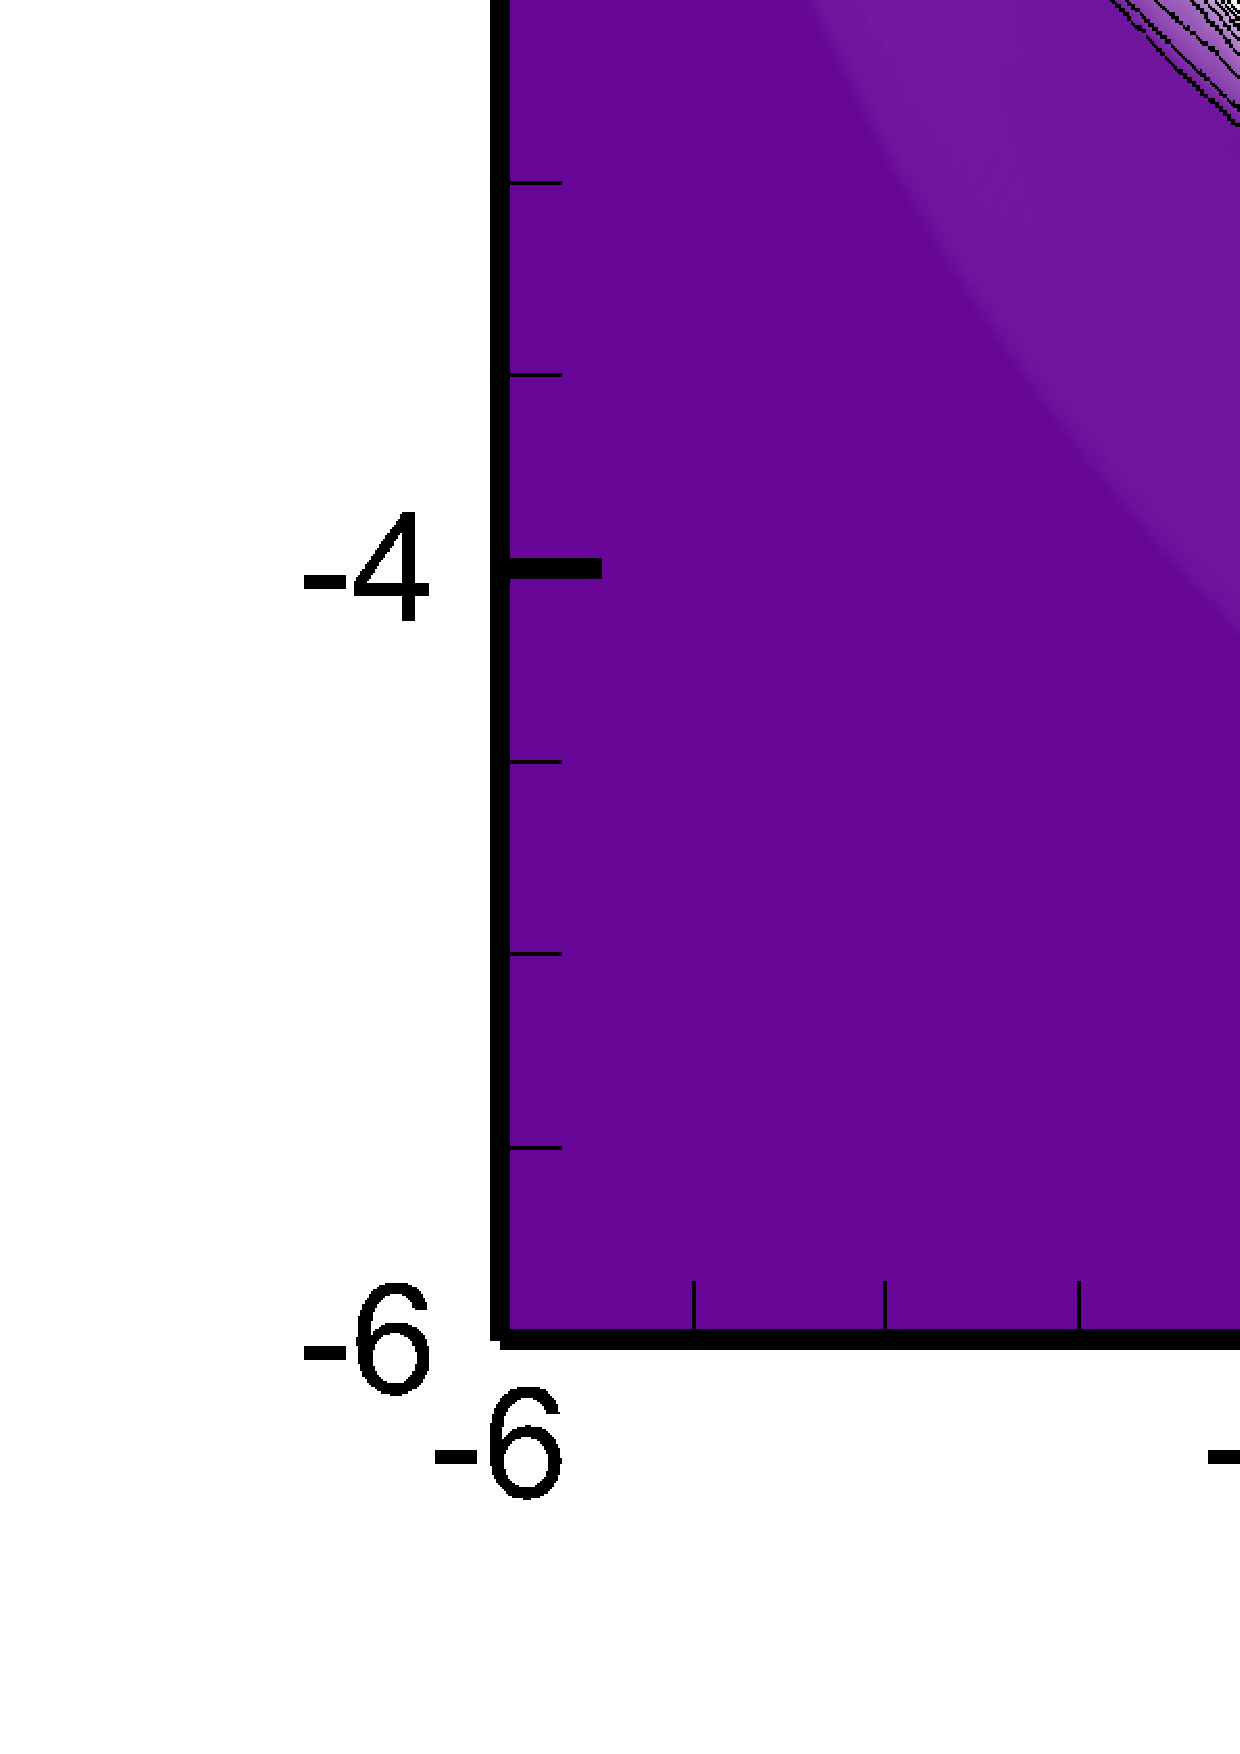
\includegraphics[width=0.33\textwidth]{grmhd-paper-official/BW_P3_Bx01_p.pdf}
%    
\includegraphics[width=0.33\textwidth]{grmhd-paper-official/BW_P3_Bx01_Lor.pdf}%
\includegraphics[width=0.33\textwidth]{grmhd-paper-official/BW_P3_Bx01_pmag_B.pdf}%

% line 2:
\includegraphics[width=0.33\textwidth]{grmhd-paper-official/BW_P3_Bx05_rho.pdf}%
\includegraphics[width=0.33\textwidth]{grmhd-paper-official/BW_P3_Bx05_Lor.pdf}%
\includegraphics[width=0.33\textwidth]{grmhd-paper-official/BW_P3_Bx05_p.pdf}%
\end{minipage}
}% end makebox

\caption[
   SRMHD blast wave, fields view \ownPub{Fambri2018}
]{Solution of the SRMHD blast wave with
  $B_x=0.1$ at time $t=4.0$, obtained with the ADER-DG $\mathbb{P}_3$
  scheme supplemented with the \textit{a posteriori}  second-order TVD subcell
  limiter. The three columns show rest-mass density $\rho$, Lorentz factor
  $\gamma$ and magnetic pressure $p_\text{mag}$.
  Published in \cite{Fambri2018}.
 }
\end{figure*}
%
%
Another standard test of the RMHD equations is represented by the 
cylindrical blast wave problem. In this benchmark, the plasma is 
initially at rest and subject to a constant magnetic field along the
$x$-direction; we have therefore considered two different configurations
strengths of the magnetic field, \ie $B_x = 0.1$ and $B_x= 0.5$,
representing the case of a moderately and of a highly magnetized plasma,
respectively.

The initial conditions for the rest-mass density and
pressure are given respectively by
%
\begin{align}
  (\rho, p ) = \left\{\begin{array}{lr} (0.01, 1)
  & \text{if} \  r<R \,, \\
  10^{-4} \times (1,5) & \text{otherwise}\,,
  \end{array}\right.
\end{align}
%
and together with the magnetic-field strength are sufficient to fully
specify the initial setup. Also in this case, and following see
\cite{Balsara1999b}, a linear smoothing is used in order to avoid sharp  
discontinuities in the initial conditions. 

The computations have been carried out in 2D with a Cartesian coordinate
system over a computational domain given by $\Omega = [-6,6]^2$, with
$40^2$ elements on the coarsest mesh level, and a maximum refinement
level $\ell_\text{max}=2$. We have used the Rusanov Riemann solver with
our ADER-DG-$\mathbb{P}_3$ scheme. The computed results for different
physical quantities, the AMR grid and the limiter status are shown in
%Fig. \ref{fig:BW_01}~ for the moderately magnetized case, and in % don't want too many figs in thesis
Fig. \ref{fig:BW_05} for the highly magnetized case. Note in the
bottom-right panels of figures the map of the ``troubled cells'' and how
these are limited in extent and nicely map the dynamics of the
discontinuities in the magnetic field. Clearly, the fraction of troubled
cells in the case of the low-magnetisation setup represent only a very
small fraction of the evolved cells (see Fig. \ref{fig:BW_05}); this
is to be contrasted with what happens in the case of the much more
challenging case of high magnetisation, where however the troubled cells
still represent less than $50\%$ of the evolved cells (see
Fig. \ref{fig:BW_05}). 

Lacking an analytic solution to compare with, the
assessment of the results in this case is harder, but it is reassuring
that the results match well those presented in other tests in the
literature, \eg by \cite{DelZanna2007,Dionysopoulou:2012pp,Zanotti2015d}.

%
\begin{figure}[t]
\makebox[\linewidth][c]{
\begin{minipage}{1.1\textwidth}
\includegraphics[width=0.5\textwidth]{grmhd-paper-official/BW_P3_Bx01_mesh.pdf}%
\includegraphics[width=0.5\textwidth]{grmhd-paper-official/BW_P3_Bx01_limiter.pdf}%

\includegraphics[width=0.5\textwidth]{grmhd-paper-official/BW_P3_Bx05_mesh.pdf}%
\includegraphics[width=0.5\textwidth]{grmhd-paper-official/BW_P3_Bx05_limiter.pdf}%
\end{minipage}
}% end of makebox
  \caption[
   SRMHD blast wave, grid \ownPub{Fambri2018}
  ]{Solution of the SRMHD blast wave with
    $B_x=0.5$ at time $t=4.0$, obtained with the ADER-DG $\mathbb{P}_3$
    scheme supplemented with the \textit{a posteriori}  second-order TVD subcell
    limiter. 
	Top panels: AMR grid, bottom panels: limiter map with troubled cells marked 
	in red and
    regular unlimited cells marked in green.
    Published in \cite{Fambri2018}.
  }
\label{fig:BW_05}
\end{figure}
%

\subsection{Orszag-Tang vortex}\label{sec:orszag-tang}
%-------------------------------------------------------------
%
%
Our final special-relativistic test of non-smooth flows is another classic
benchmark represented by the relativistic version of the Orszag-Tang
vortex system \cite{Orszag1979}. This is a useful application of our
numerical infrastructure as it involves the development of a complex and
non-smooth magnetic-field structure and hence it explores geometries
without trivial symmetries.

The initial conditions in this case are given by the vector of conserved
variables 
%
\begin{equation*}
%\label{eq:OrszagTang_ic}
\left( \rho, u, v, w, p, B_x ,B_y,B_z \right) = \left( 1 , -
  \frac{3}{4\sqrt{2}}\sin y\,, \frac{3}{4\sqrt{2}}\sin x \,, 0, 1, - \sin
  y\,, \sin 2x \,, 0 \right)\,,
\end{equation*}
%
with $\Gamma=4/3$. The computational domain is $\Omega = [0,2\pi]^2$,
with $30^2$ elements on the level-zero grid, a maximum refinement level
of $\ell_{\text{max}}=2$, periodic boundary conditions and a Rusanov
Riemann solver for the subcell finite-volume limiter.

Figure \ref{fig:OrszagTang} shows the numerical results for the AMR grid {
with limiter status, the rest-mass density and the divergence-cleaning scalar 
$\psi$ at different times, together}
with the corresponding numerical solution obtained with the same scheme
on a fine uniform $270^2$ mesh, corresponding to the finest mesh
resolution at $\ell=\ell_{\text{max}}$ and which serves here as a
reference. The figure, in particular, refers to simulations in which the
$\mathbb{P}_5$-version of our ADER-DG has been adopted. Also for this
test, a rigorous accuracy analysis is not trivial but we note the very
good agreement between the AMR simulations and the fine uniform-grid
reference solution, as well as with the corresponding solutions that
are published in \cite{Zanotti2015d,Porth2017}. 
Note also how the AMR grid structure and the troubled-cells
patterns closely follow the development of steeper gradients and 
discontinuities.

%
\begin{figure*}
\makebox[\linewidth][c]{%holding 3 figures next to each other
	\begin{minipage}{19cm}
	\includegraphics[width=0.32\textwidth]{grmhd-paper-official/OT_t30_p.pdf}%
	\includegraphics[width=0.32\textwidth]{grmhd-paper-official/OT_t30_limiter.pdf}%
	\includegraphics[width=0.32\textwidth]{grmhd-paper-official/OT_t30_psi.pdf}%
	
	\includegraphics[width=0.32\textwidth]{grmhd-paper-official/OT_t70_p.pdf}%
	\includegraphics[width=0.32\textwidth]{grmhd-paper-official/OT_t70_limiter.pdf}%
	\includegraphics[width=0.32\textwidth]{grmhd-paper-official/OT_t70_psi.pdf}%
    \end{minipage}
}% end of makebox
	\caption[
	SRMHD Orszag-Tang vortex \ownPub{Fambri2018}
	]{SRMHD Orszag-Tang vortex problem at times
		$t=3$ (upper row) and $t=7$ (lower row), obtained through
		the ADER-DG-$\mathbb{P}_5$ scheme supplemented with the \textit{a 
		posteriori} 
		TVD subcell limiter on a $30^2$ elements on the coarsest grid
		($\ell=0$), two maximum refinement levels and a refinement factor
		$\mathcal{R}=3$. Color encoded, from left to right, are:
		Rest mass density $\rho$, AMR grid and limiter status,
		divergence cleaning scalar $\psi$.
	    Published in \cite{Fambri2018}
    }
	\label{fig:OrszagTang}
	\\
\end{figure*}
%

%=============================================================
\section{Non-smooth general-relativistic benchmarks}
\label{sec:discontinuous_gr}
%=============================================================

In the following two sections we discuss the use of our ADER-DG method in
non-smooth general-relativistic flows, either in 2D and spherical
coordinates or in 3D and Cartesian coordinates. The tests involve the
evolution of non-selfgravitating tori as those presented in
Sec. \ref{sec:discontinuous_sr} with the important difference that the
computational domain here fully contains the torus, whose exterior is
therefore filled with a uniform atmosphere at a rest-mass density of
$\rho_0=10^{-9}$ that is five orders of magnitude smaller than the one at
the torus centre.

%-------------------------------------------------------------
\subsection{2D torus around a Schwarzschild black hole}
\label{sec:full_torus}
%-------------------------------------------------------------

First, we consider a thick torus in equilibrium orbiting around a
black-hole with the parameters previously described in
Sec. \ref{sec:2D_torus_interior} and using horizon-penetrating spherical
KS coordinates in 2D. The computational domain $(r,\theta) \in \Omega =
[2,18] \times[0.5,2.5]$ is discretized with a uniform mesh of $50^2$ 
elements using an ADER-DG-$\mathbb{P}_3$ scheme with TVD subcell 
finite-volume limiter (as a comparison, the torus has an inner radius 
$r_{\rm in} = 5.5M$ and an outer radius $r_{\rm out}= 13.8M$, so that 
the entire torus is resolved with only 26 elements in radial direction
and 14 elements in angular direction). 
On the outer edge we impose the initial data as boundary condition in all 
variables. 

A 1D cut of the rest-mass density in the radial direction is shown in the
left panel of Fig. \ref{fig:Torus.cut} and is plotted over the analytic
solution at $t=100\,M$.  Note the excellent agreement between the
numerical results and the exact solution, with differences in the central
rest-mass density that are less than $0.7\%$.

\begin{marginfigure}
\makebox[\linewidth][c]{%holding 3 figures next to each other
\begin{minipage}{1.2\textwidth}
	\includegraphics[width=1.1\linewidth]{grmhd-paper-official/Torus2D-cut-t100.pdf}
	%     & 
	\includegraphics[width=1.1\linewidth]{grmhd-paper-official/Torus3D_KSC_P3_1Dcut_t30.pdf}
\end{minipage}
}% end makebox
	\caption[
	Radial tori plots \ownPub{Fambri2018}
	]{Radial 1D cut of the thick torus, comparision of the ADER-DG 
		$\mathbb{P}_3$ solution with second-order TVD subcell limiter
		after $t=100$M compared with exact solution. The right panel
		shows different azimuthal angles.}
	\label{fig:Torus.cut}
	%\end{center}
\end{marginfigure}

It is useful to remark that the low-density atmosphere has been
successfully simulated and robustly evolved in time with a high-order
ADER-DG scheme and that inside the computational domain the limiter is 
activated only on the border of the torus, where 
spurious oscillations may generate possibly negative-valued densities and
pressures in the high-order DG polynomials. However, the {a-posteriori}
subcell finite-volume limiter appears to be robust enough to accurately
treat the atmosphere of the torus. Furthermore, we note that the fluid in
this low-density region is treated so as to be evolved as a standard
fluid, \ie the velocity is not set to zero in a computational cell that
is marked to host the atmosphere. As a result, during the simulations,
the atmosphere the fluid in the atmosphere starts accreting onto the
black hole; in practice the amount of matter accreted in this manner is
minute and does not influence with the dynamics of the much denser matter
lost from the torus.


%-------------------------------------------------------------
\subsection{3D torus around a Schwarzschild black hole}\label{sec:3d-torus-gr}
%-------------------------------------------------------------
In this section, a fully 3D evolution of the torus (from the previous
section) is considered, \ie the azimuthal spatial dimension is added.

For this, we use a horizon-penetrating Cartesian KS coordinates which
cover a computational domain chosen to be $(x,y,z) \in \Omega = [-18,+18]
\times [2,18]\times[-8,+8]$. The portion of the domain around the origin
is excised following the same logic discussed in sec. \ref{sec:3D_Michel}.
 The solution has been computed using an
ADER-DG-$\mathbb{P}_3$ scheme on a uniform mesh composed of
$40\times20\times20$ elements.  

The 1D cut of the rest-mass density profile on the equatorial plane
$\theta=\pi/2$ and along different angular directions $\phi=\pi/4$,
$\pi/2$ and $3 \pi/4$ at $t\sim 30\,M$.  The various numerical solutions
are overlayed with the corresponding analytic solutions in the right
panel of Fig. \ref{fig:Torus.cut}. Once again, we can observe an
excellent agreement between numerical and exact solution, with
differences in the central rest-mass density that are less than $1.5\%$.

\subsection{Preliminary results on a TOV star}\label{sec:tov}
The Tolman-Oppenheimer-Volkoff (TOV) solution of general relativity is a popular choice
for modelling neutron stars. It is a spherically symmetric static spacetime of
an isotropic fluid in equilibrium. For such an energy momentum tensor, Einstein
equations reduce to the TOV equations \cite{Tolman39,Oppenheimer39b}
\begin{equation}
\dd pr=-\frac{\rho\, m(r)}{r^2}\left(1+\frac{p}{\rho}\right)\left(1+\frac{4\pi r^3 \,p}{m(r)}\right)\left(1-\frac{2}{r}\right)^{-1}
\end{equation}
where $m(r)=\int_0^r 4\pi\tilde r^2 \rho \d \tilde r$ is the total mass within a shell of
radius~$r$. TOV equations can be solved numerically, \ie solve the system in favour
of a requested total mass $M=\lim_{r\to\infty}m(r)$ or a requested central hydrodynamic
quantity such as the central density $\rho_0$. However, the full arsenal of GR
approximations (Section \ref{sec:gr-intro}) can be applied to TOV equations, such as
Post-Newtonian approximations.

In this test, we created initial data for a 1.45$\Msol$ neutron star with
radius $R=5.84 \Msol = 8.6$km in isotropic coordinates and central rest mass density
$\rho_c = 1.28\times 10^{-3} \Msol^{4} = 4.9 \times 10^{18}$kg/m$^3$,
described by a polytropic EOS with $\Gamma=2, K=100$ (in geometric units). The initial
can be solved with an arbitrary numeric \code{TOVSolver}
\footnote{
	See Appendix~\ref{apx.codes} for a list of ODE solver codes which
	where used within this text.
}. The star is evolved in full 3D on a domain with an extend of at least 
$\Omega=[-10\Msol,10\Msol]^3$ with outflow (copy) boundary
conditions on all boundaries.

While the interpolation of the initial data on the evolution grid always adds a little
perturbation, an additional well-defined ``physical'' perturbation should be added
which produces deterministic results in a code comparison.

Our findings are presented in Figure~\ref{fig:tov-preliminary}. Here, we compare a
1\% pressure perturbation evolved with \code{WhiskyTHC}
\cite{Radice2013,Radice2015},
\ie a finite differencing code, vs. the ADER-DG code, but with artificial viscosity
turned on. One can clearly see that the artificial viscosity, which shall avoid the
activation of the limiter at the surface, damps all errors, artificially stabilizes
the simulation but removes the physical modes (vibrations) which characterize the star.
\todo[color=green]{TOV star: Probably write more about TOV star and preliminary results}

\begin{figure*}[t]
	\includegraphics[width=\textwidth]{tovmodes-preliminary/tovmodes-preliminary.pdf}
	\caption[
	  TOV preliminary data \exclusive
	]{Evolution of central density error (left panel), vs. power density
      spectrum (norm of fourier transform, right panel) of the two curves,
      with the frequency of peaks predicted by perturbation theory marked in red.
      The figure shows two codes compared to each other. The better the peaks
      are reproduced, the better the code performs in this test.
     }\label{fig:tov-preliminary}
\end{figure*}

\section{Summary}
In the present Chapter~\ref{chapter:hydro}, the equations of general 
relativistic magnetohydrodynamics (GRMHD) have been reviewed and casted in
a form with conserved and nonconserved fluxes. In a couple of static spacetime
benchmark scenarios, their correct implementation with a sophisticated ADER-DG
scheme, presented in section~\ref{sec:dg}, is demonstrated. Preliminary
results on astrophysically interesting scenarios, such as the TOV star,
were given.

